
\section{Evaluation}

\subsection{Data-Driven Performance Engineering}
\subsubsection{Sparse-Sparse Matrix Multiply}

\help{The main points of this section are:}

\help{1. summarize the difference between inner, gustavson, and outer, cite gamma but this also needs to stand on it's own}


\help{2. Explain why bytemap temporary makes sense for gustavson, but not for outer or inner}

\help{3. Point out that TACO does not even support outer product because it does not support scatter into 2D workspace}

\help{4. Take a look at the figure and point out that Finch is competitive with TACO on inner and gustavson, and that for outer product we see what we would expect from TACO: i.e. Finch Outer with dense performs similarly to TACO with dense, and Finch Outer with sparse performs much better as the matrix size increases.}

\help{5. point out that for the large matrices finch is competitive with TACO for gustavson}.

\help{6. explain the features of "datastructure-driven programming" that are used here in this problem. i.e. explicit temporary, bytemap format, transpositions}.
\begin{figure}
	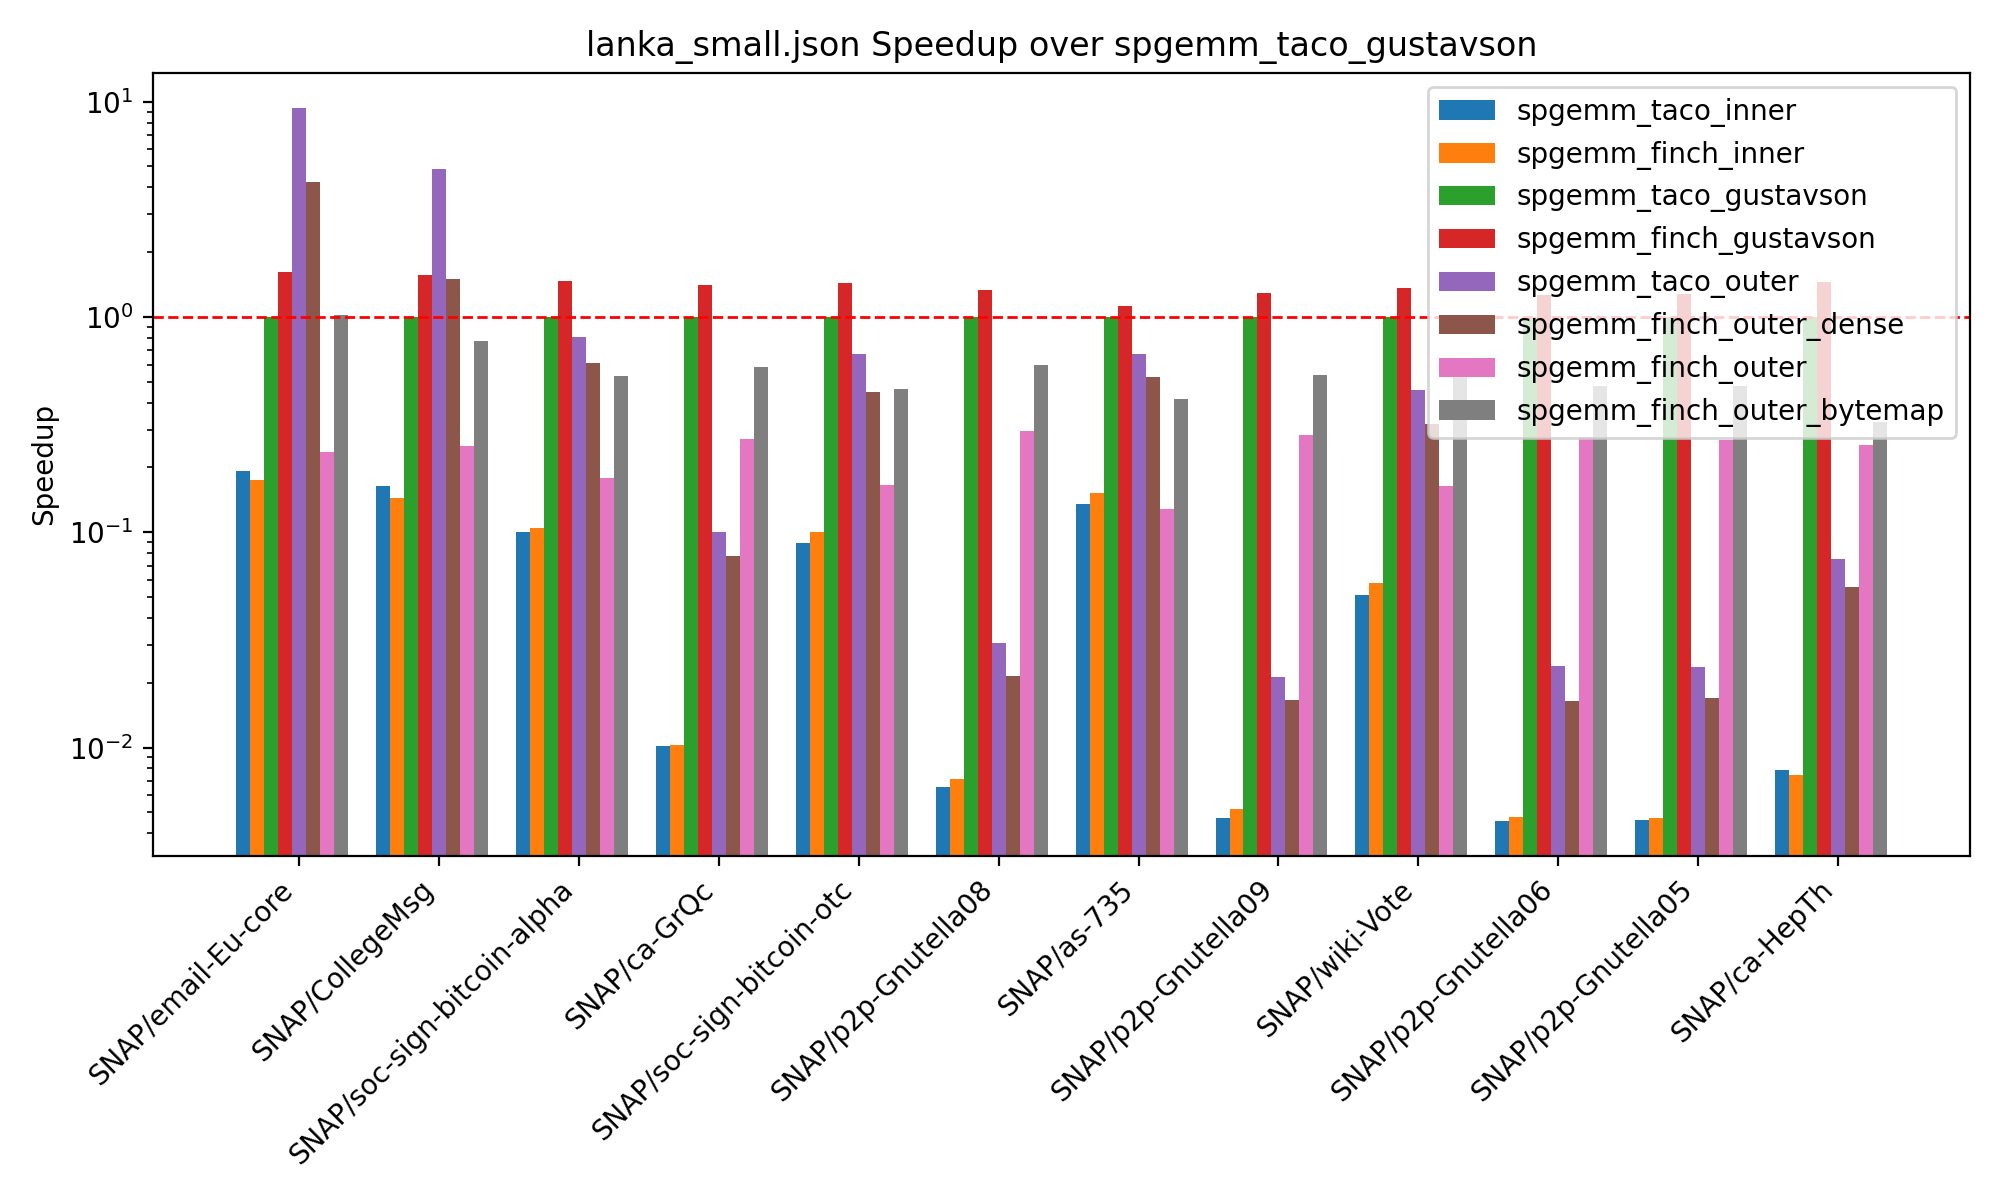
\includegraphics[width=\linewidth]{spgemm_small_speedup_log_scale.png}
    \caption{A comparison of several matrix multiplication algorithms between Finch and Taco smaller matrices, ordered from small to big dimension. Note that inner products necessarily requires $O(n^2)$ work and taco's outer products format is dense. Finch can use a sparse outer products format and thus has an asymptotic advantage that becomes evident as the output dimensions grow.}
\end{figure}

\begin{figure}
	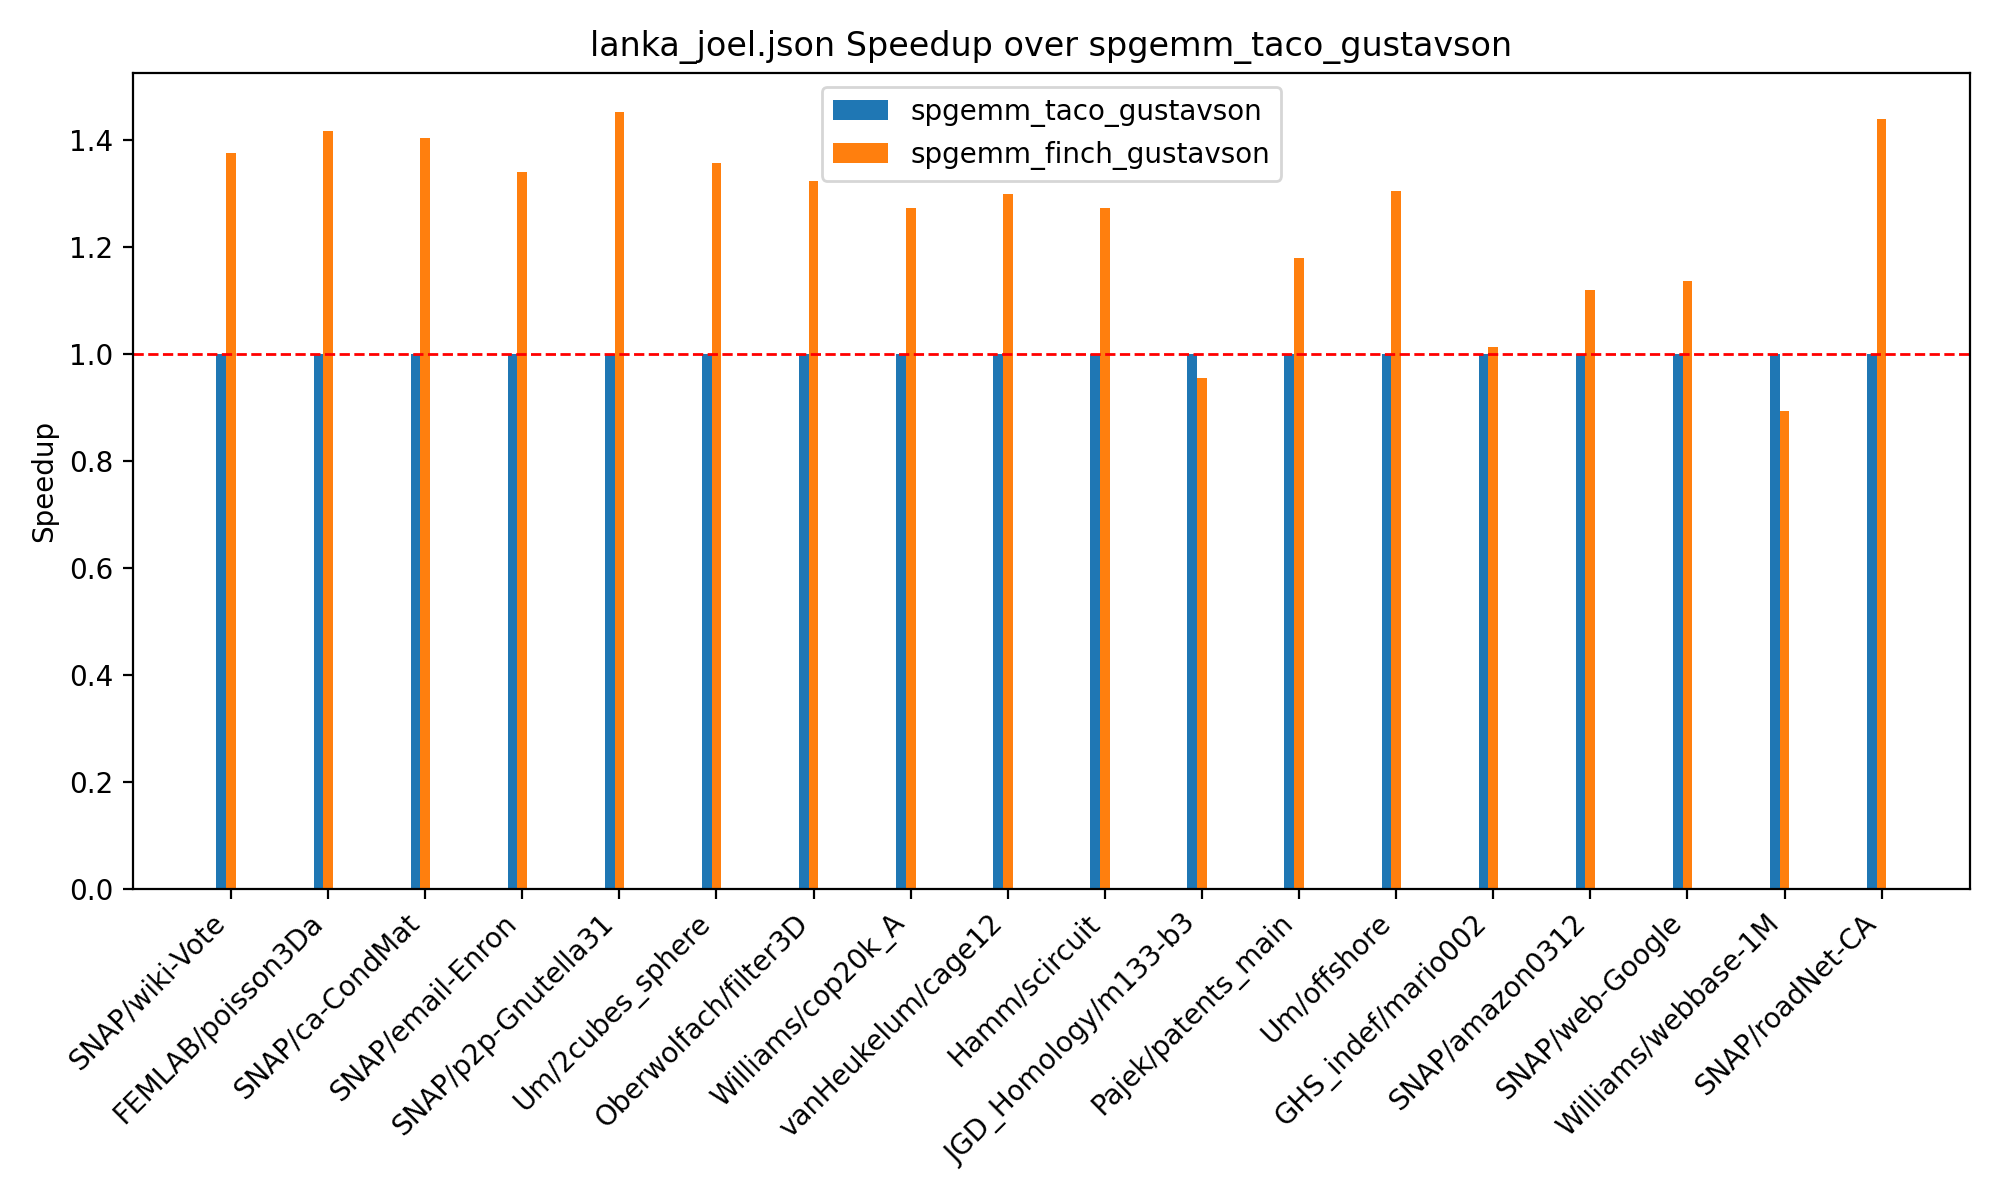
\includegraphics[width=\linewidth]{spgemm_joel_speedup.png}
    \caption{A comparison of gustavson's algorithm between Finch and Taco on some larger matrices}
\end{figure}

Examples that demonstrate performance engineering in a datastructure-driven model

\subsubsection{SpMV}
Finch provides many flexible level formats to efficiently capture a variety of patterns in datasets, encompassing both the structure and type of data. More specifically, these formats can represent banded, triangular, run-length-encoded, blocked, hashed, and boolean data, as well as several other formats. Finch also provides the control flow necessary to manipulate the order in which data in these flexible level formats is read and written, enabling us to take advantage of multiple structural patterns concurrently—for example, we can exploit both sparsity and symmetry by using a sparse level format and restricting data reads to one triangle of a matrix. % I'm not sure if the right place for this is here - maybe should come earlier?

Structure in data arises both naturally, due to the chemical and physical properties of matter, and artificially via mathematical operations that induce particular patterns. Closely tailoring a storage format to a particular data pattern enables us to reduce the amount of stored values, make data accesses more efficient, and take advantage of spatial locality, resulting in more performant code.

The sparse matrix-vector multiplication kernel is a common operation in sparse linear algebra with many applications including conjugate gradients, graph algorithms, numerical analysis, and neural networks. The wide range of applications unsurprisingly results in a wide range of types of datasets making it an effective kernel to demonstrate the utility of having flexible data formats. In this case study, we highlight a few different Finch formats and the performance effects of conforming a dataset’s structure with its storage format, which Finch's datastructure-driven model enables us to do.

We compare Finch’s performance to that of TACO, SuiteSparseGraphBLAS, and Julia’s standard library.  We test using sparse matrices from a large selection of datasets spanning several previous papers: the datasets used by Vuduc et al. to test the OSKI interface [cite], Ahrens et al. to test a variable block row format partitioning strategy [cite], and Kjolstad et al. to test the TACO library [cite]. In addition, we also created several synthetic matrices containing bands or blocks of varying sizes as well as a permutation matrix to encapsulate a few additional use cases. The dense vector is randomly generated. We depict the performance of SpMV across the aforementioned tools and compare to the fastest Finch format for that particular dataset in Figures 1 and 2. 

% TODO: make this be 3 columns
\begin{figure}
    \begin{minipage}[t]{0.315\textwidth}
        \vspace{0pt} % Add this to ensure top alignment within minipage
        \begin{minted}{julia}
            @finch begin
                y .= 0
                for j = _, i = _
                    y[i] += A[i, j] * x[j]
                end
                return y
            end
        \end{minted}
    \end{minipage}%
    \begin{minipage}[t]{0.315\textwidth}
        \vspace{0pt} % Add this to ensure top alignment within minipage
        \begin{minted}{julia}
            @finch begin
                y .= 0
                for j = _, i = _
                    y[j] += A[i, j] * x[i]
                end
                return y
            end
        \end{minted}
    \end{minipage}
    \begin{minipage}[t]{0.36\textwidth}
        \vspace{0pt} % Add this to ensure top alignment within minipage
        \begin{minted}{julia}
            @finch begin
                y .= 0
                for j = _
                    let x_j = x[j]
                        y_j .= 0
                        for i = _
                            let A_ij = A[i, j]
                                y[i] += x_j * A_ij
                                y_j[] += A_ij * x[i]
                            end
                        end
                        y[j] += y_j[] + diag[j] * x_j
                    end
                end
                return y
            end
        \end{minted}
    \end{minipage}
    \caption{Performance of SpMV across various tools.}
\end{figure}

\subsubsection{Tensor Formats}
We benchmarked the SpMV kernel using the Dense level format for the outer level and the SparseList, SparseVBL, SparseBand, and SparsePoint Finch levels for the inner level of the sparse matrix. To represent scalar values, we benchmarked with both the Element and Pattern levels. The SparseList, SparseVBL, and SparseBand formats were functional for all matrices, but the SparsePoint format was applicable only for the synthetic permutation matrices. The Element format was applicable to represent scalars in all matrices, while the Pattern level was applicable only for boolean matrices. 

We found that the SpMV performance was superior for the level format that best paralleled the structure of the tensor. Namely, matrices with a clear blocked structure like $exdata\_1$, $TSOPF\_RS\_b678\_c1$, and $heart3$ performed notably well with the SparseVBL format in comparison to both TACO and the Finch SparseList formats (which we consider the closest analog to the sparse matrix format used in TACO and other libraries) with speedups of 2.16, X, and Y relative to TACO and of 1.47, X, and Y relative to the SparseList Finch SpMV implementation. Furthermore, the synthetic Toeplitz banded matrices we constructed performed the best with the SparseBand matrix, in particular with the $toeplitz\_large\_band$ and the $toeplitz\_medium\_band$ matrices having a speedup of A and B relative to TACO and a speedup of A and B relative to the SparseList Finch SpMV implementation. 

There were also significant advantages of using the Pattern format instead of the Element format to represent scalar values in the matrices when these values were boolean. The matrices in the SNAP collection which represent graph datasets are boolean and had an average speedup of X over TACO and X over the same Finch program, but with an Element format.   


\subsubsection{Symmetric SpMV}
Finch enables us to exploit symmetry in the sparse matrix of the SpMV kernel by providing the capabilities to reuse memory reads and insert control flow logic to restrict iterations to either the lower or upper triangle of the sparse matrix. We can apply this strategy with any level format. Every symmetric matrix in the SparseList and SparseList-Pattern formats has better performance when we use a Finch SpMV program that takes advantage of this symmetry. However, the regular Finch SpMV program has better performance for symmetric matrices than the symmetric Finch SpMV program for the other more specialized formats, likely because we need in-order accesses to fully capitalize on the specialized storage. Symmetric SpMV with the SparseList level format in Finch results in an average of 1.3x speedup over TACO and symmetric SpMV with the SparseList-Pattern format in Finch results in an average speedup of 1.15x over TACO . Notably, there is a 1.9x speedup for the HB/saylr4 matrix. 
\subsubsection{4D Blocked SpMV}



%Here's a figure with spmv_performance_sorted_(faster_than_taco).png and spmv_performance_sorted_(slower_than_taco).png

\begin{figure}
    \begin{minipage}[t]{0.5\textwidth}
        \vspace{0pt} % Add this to ensure top alignment within minipage
        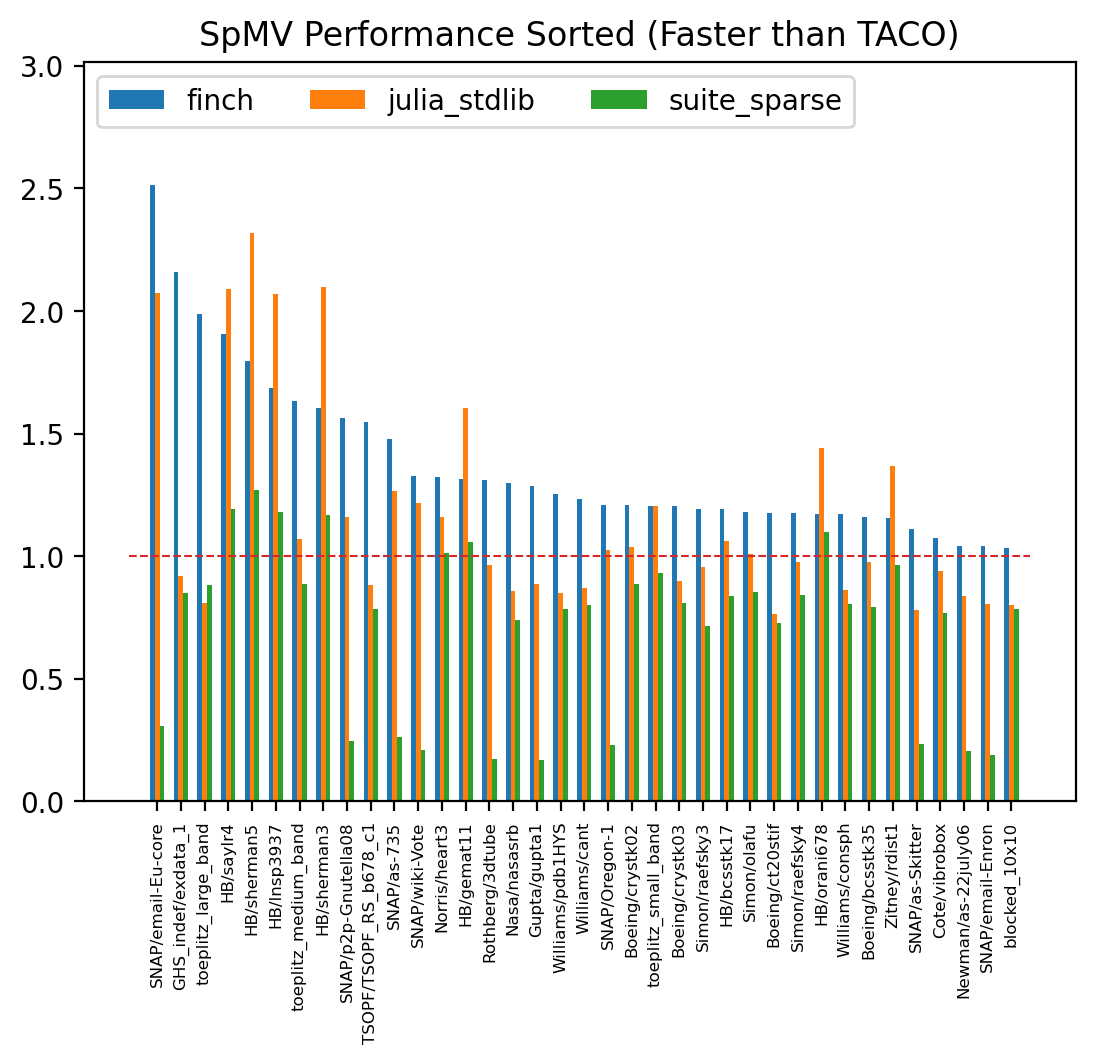
\includegraphics[width=\linewidth]{spmv_performance_sorted_(faster_than_taco).png}
    \end{minipage}%
    \begin{minipage}[t]{0.5\textwidth}
        \vspace{0pt} % Add this to ensure top alignment within minipage
        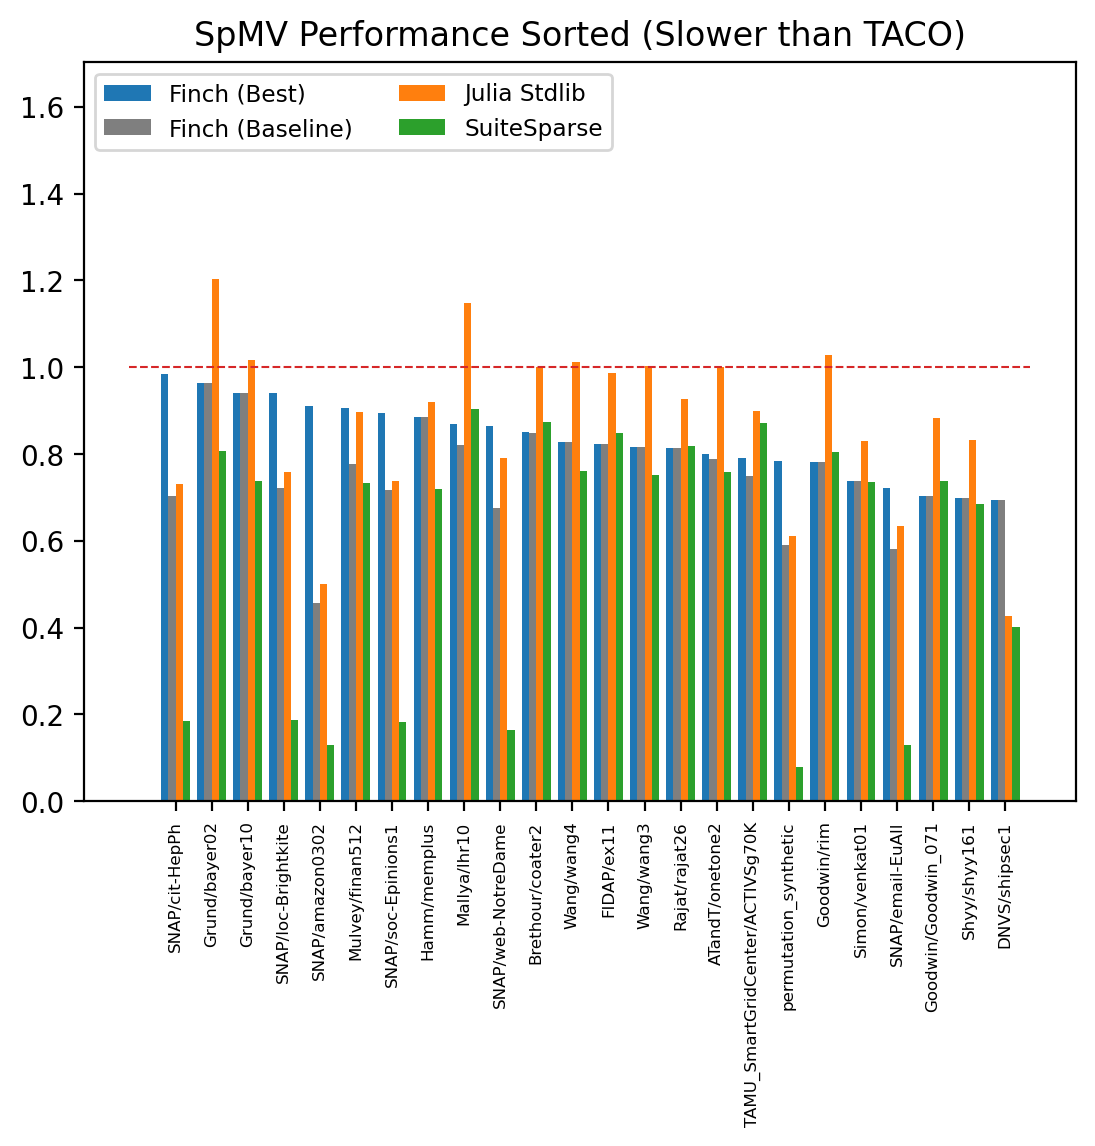
\includegraphics[width=\linewidth]{spmv_performance_sorted_(slower_than_taco).png}
    \end{minipage}
    \caption{Performance of SpMV across various tools.}
\end{figure}

\begin{figure}
    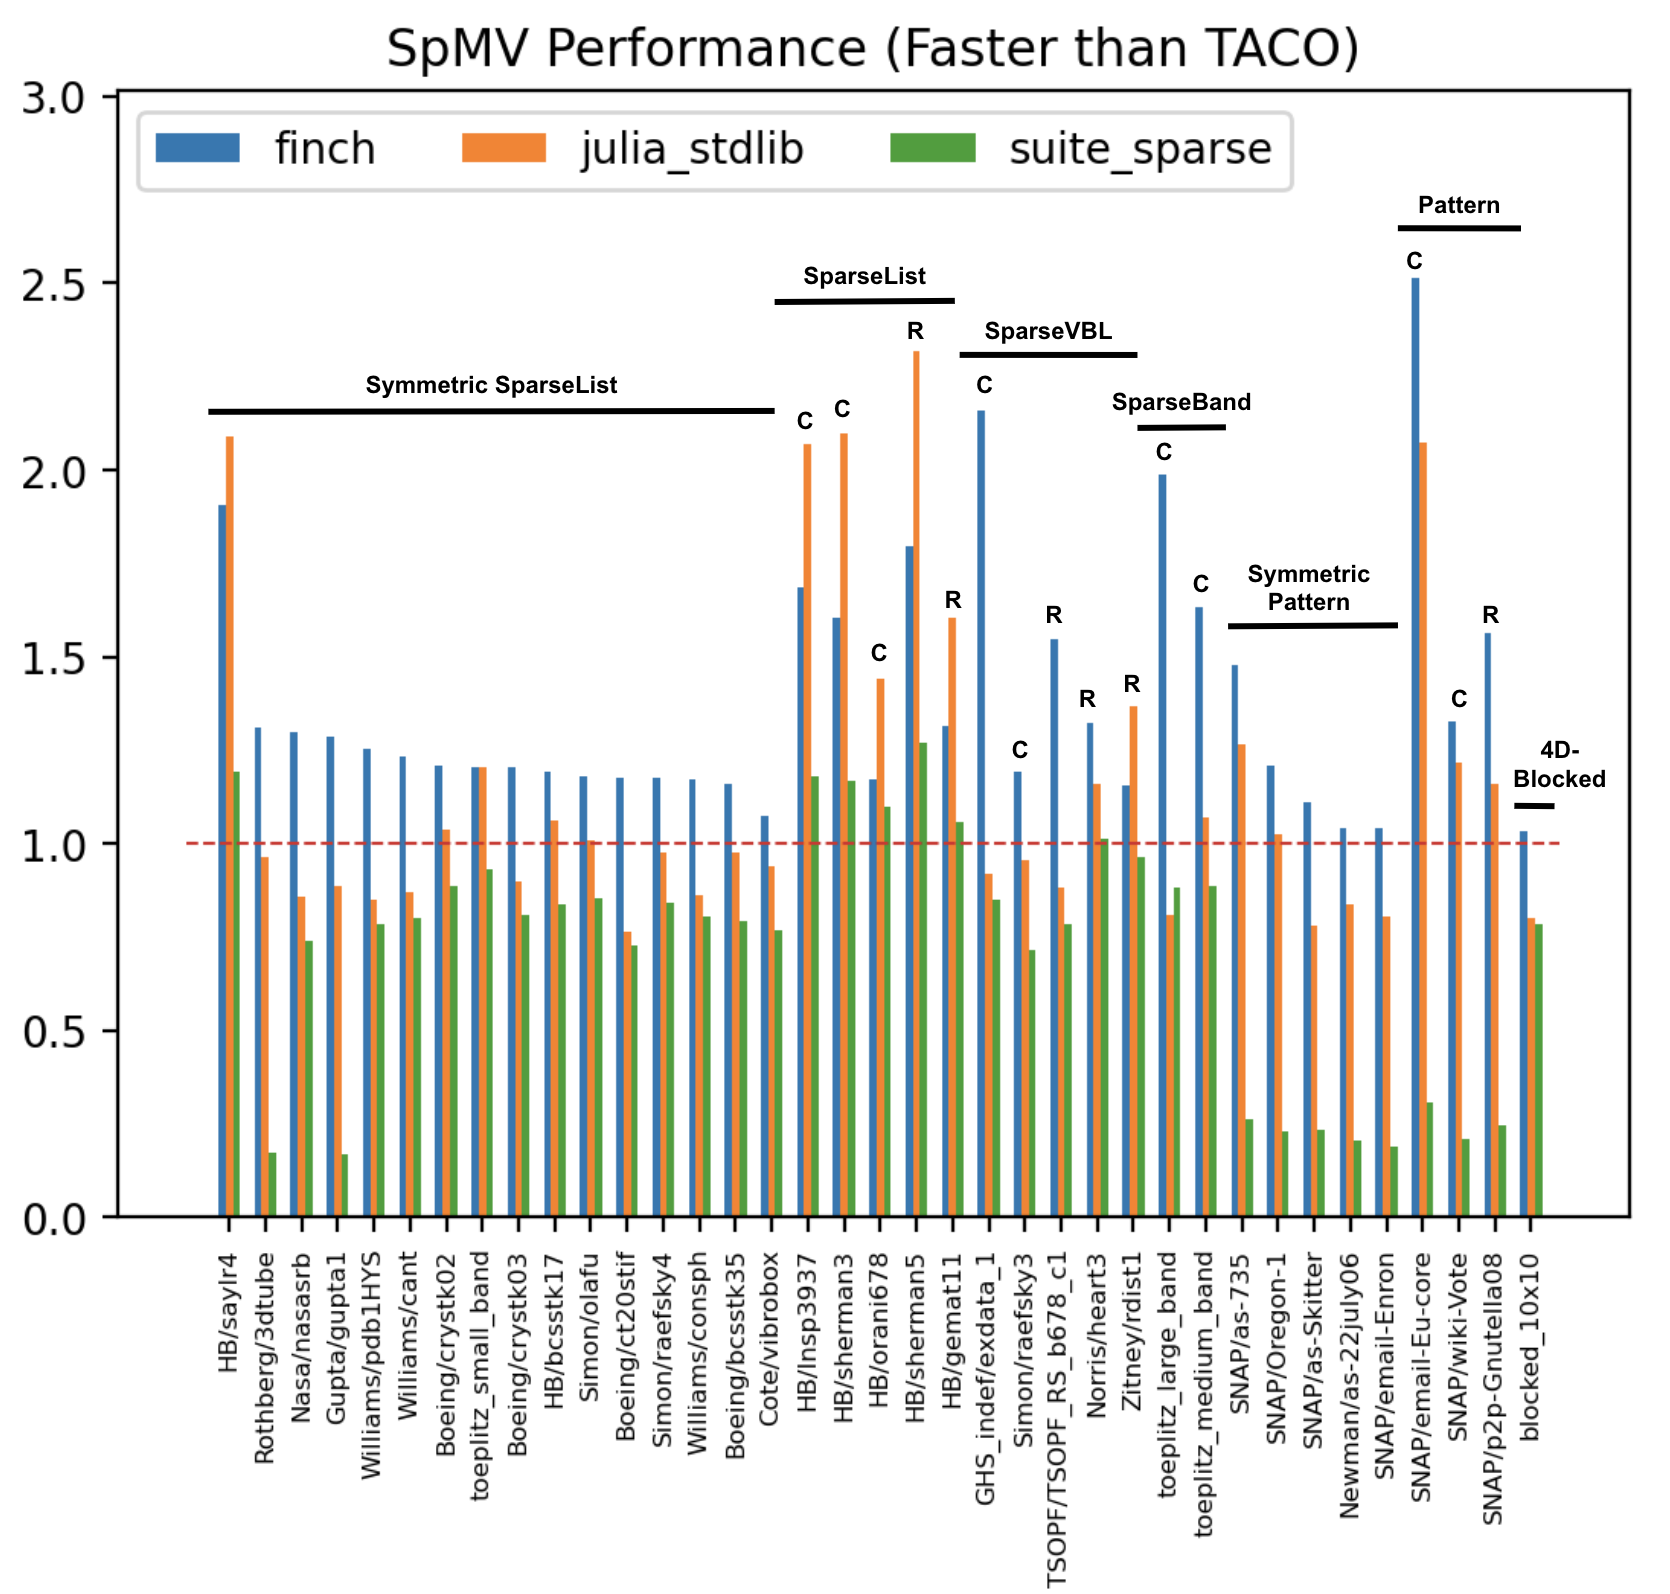
\includegraphics[width=\linewidth]{spmv_performance_grouped.png}
    \caption{Performance of SpMV by Finch format.}
\end{figure}

\subsection{Programming over flexible data}

\subsubsection{Image Morphology}

\help{In this section, explain what erosion is, link a few cool images that show erosion, and then explain what the finch kernel looks like. in particular, be sure to point out that we're doing unrolled convolution, and how that maps to the generated code (merging shifted sparse iterators).}

\help{Explain the role of formats in this kernel, how sparseRLE(PAttern) is really the right thing to use here}

\help{Explain that finch can support a bitwise version, and that finch can mask the bitwise kernel too to get performance with a small change to the code}

\help{Point out that masks with SparseRLE can sometimes perform better because they lift the masking out of the inner loop. Talk about hist and also the fact that Finch supports scatter, here and in spgemm.}

\begin{figure}
	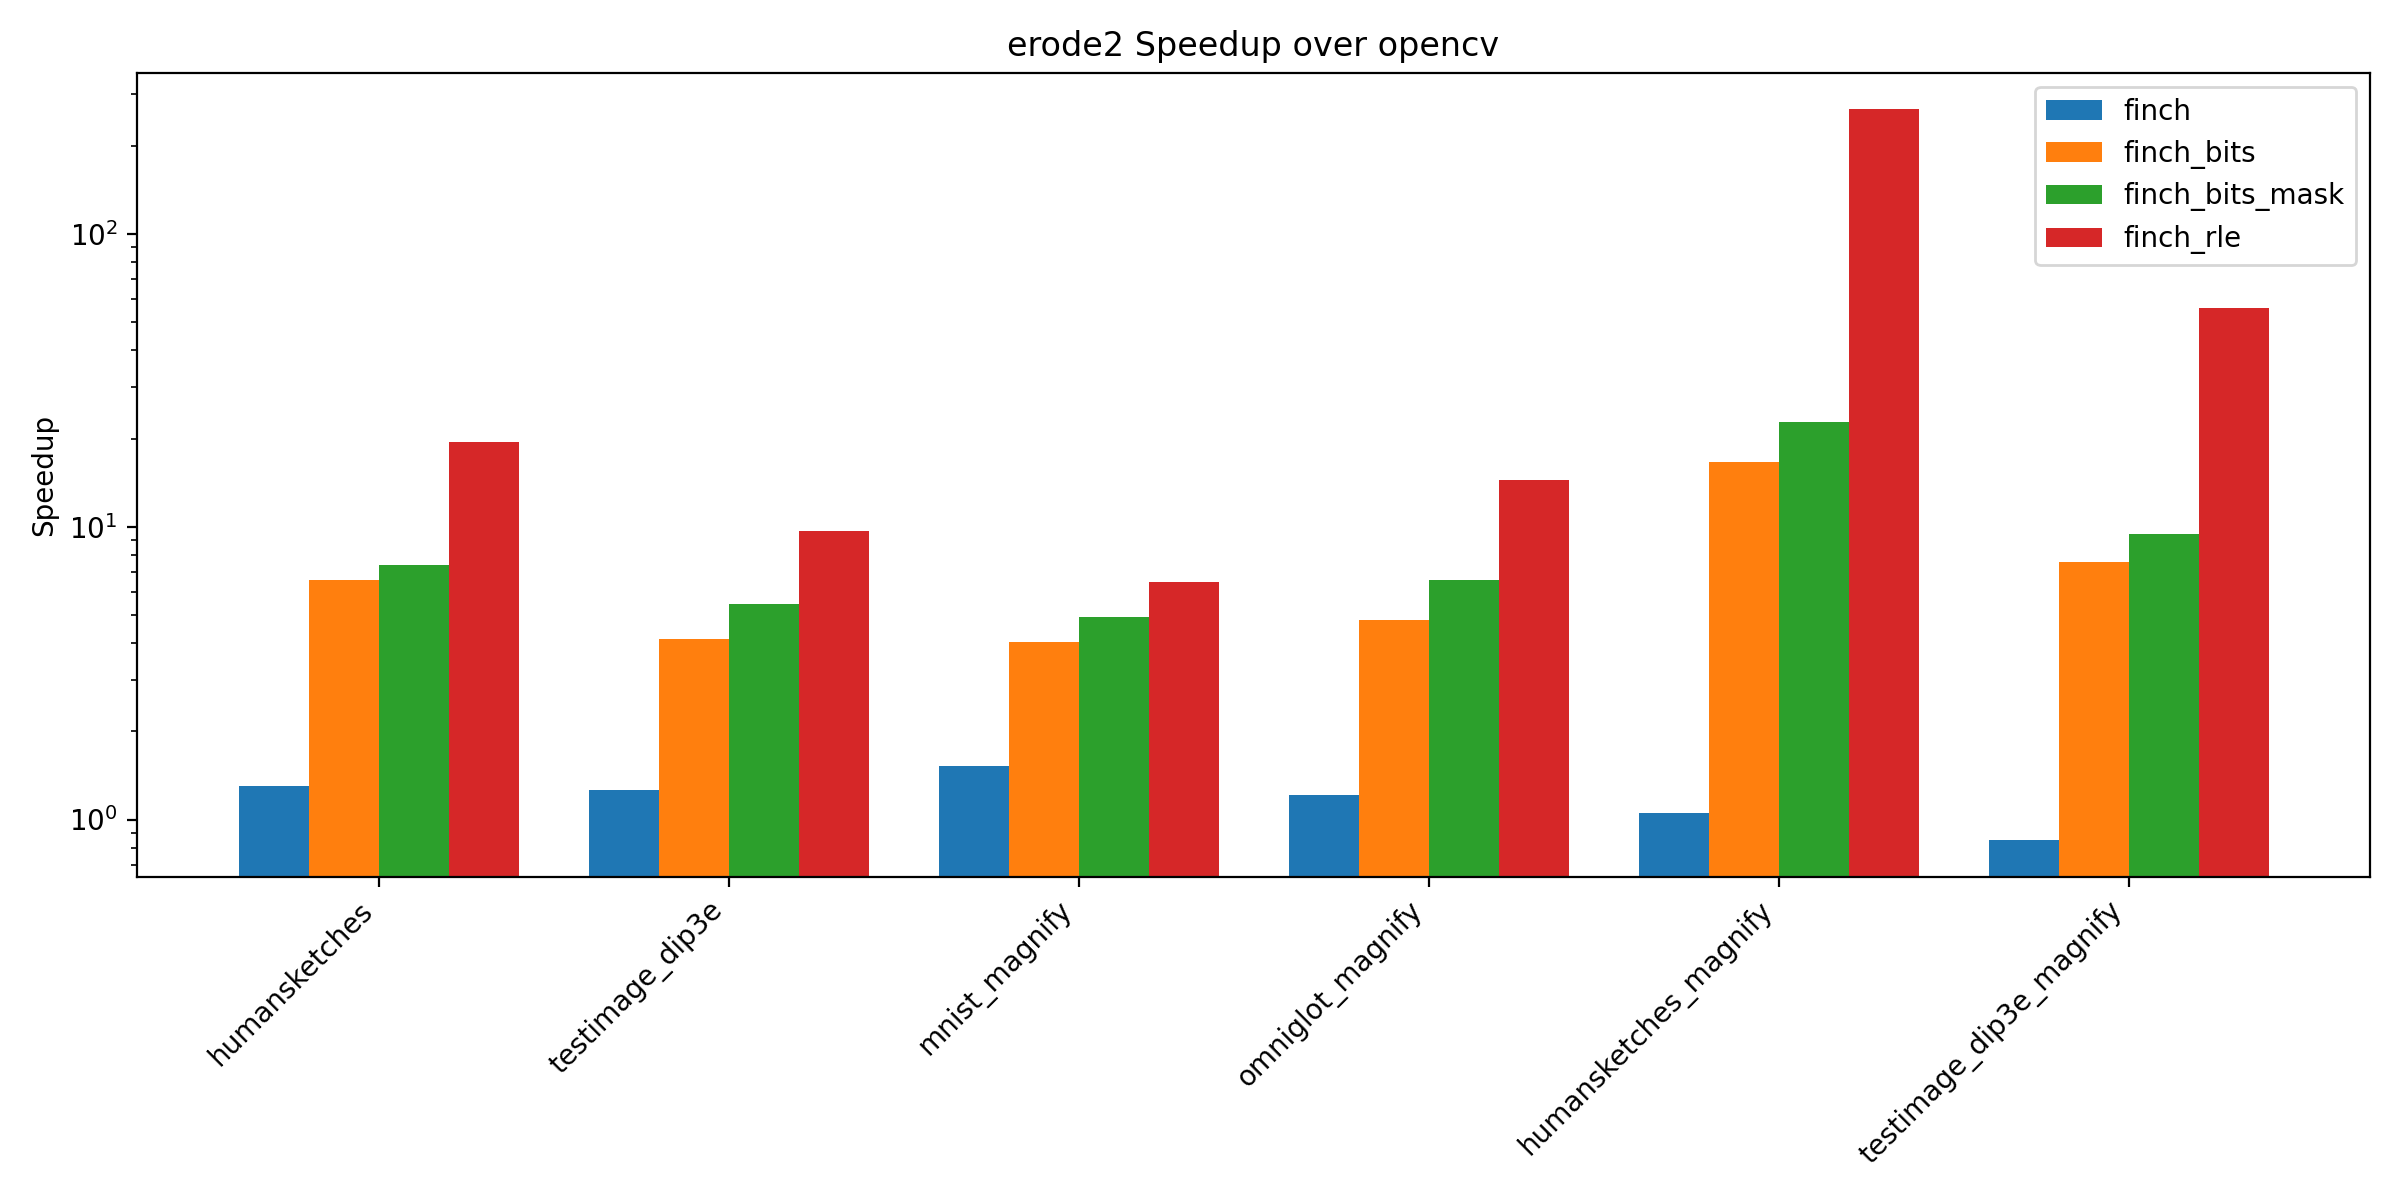
\includegraphics[width=\linewidth]{erode2_speedup_over_opencv.png}
    \caption{Performance of Finch on erosion task (2 iterations).}
\end{figure}

\begin{figure}
	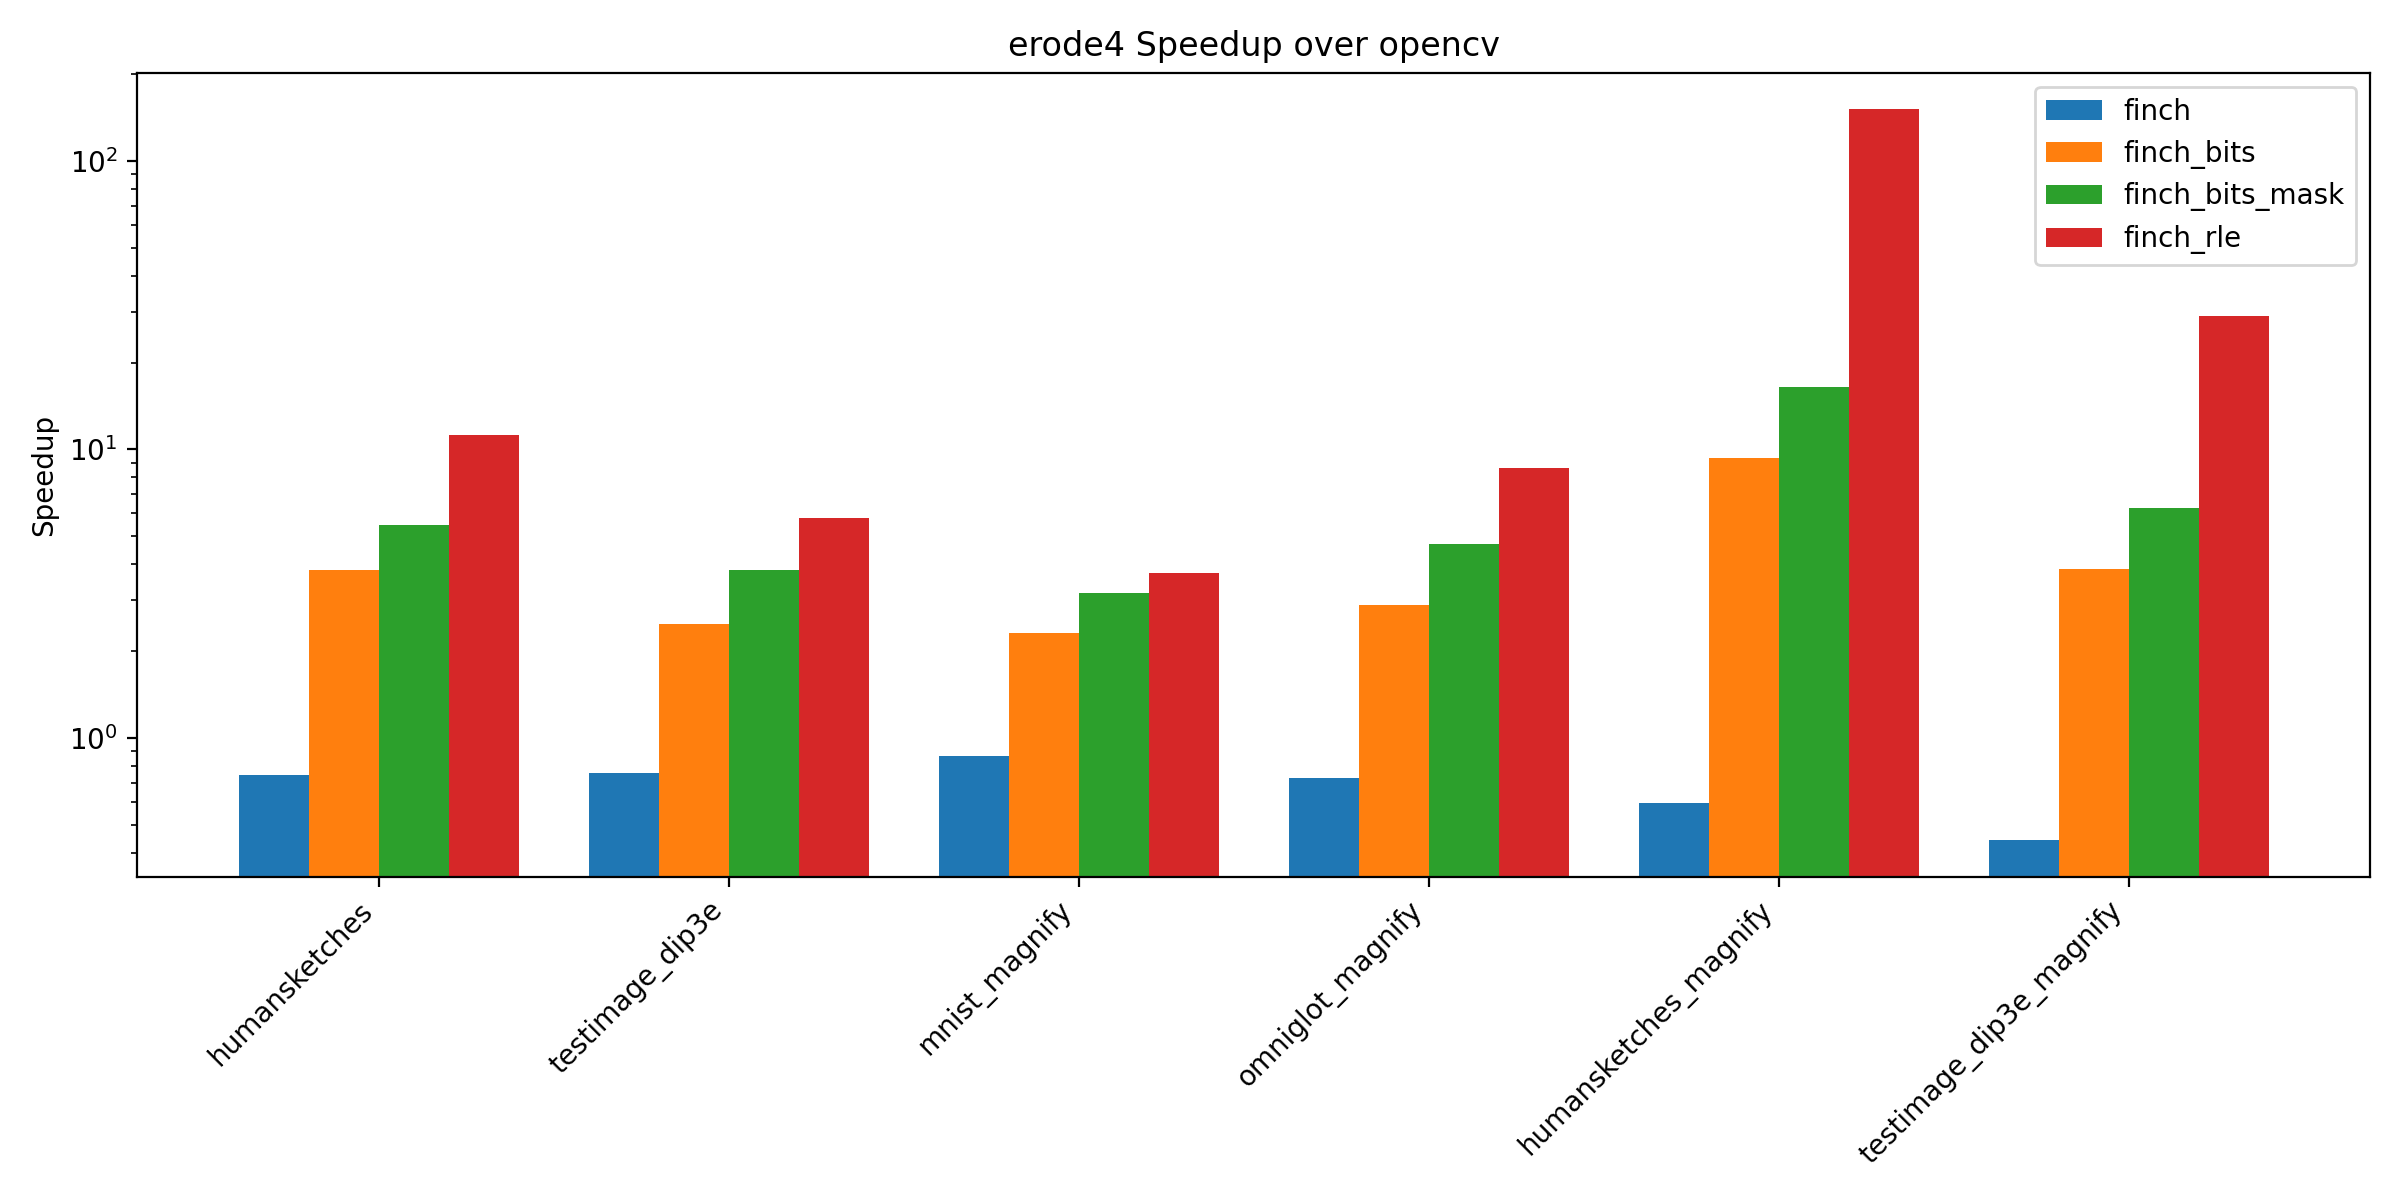
\includegraphics[width=\linewidth]{erode4_speedup_over_opencv.png}
    \caption{Performance of Finch on erosion task (4 iterations).}
\end{figure}

\begin{figure}
	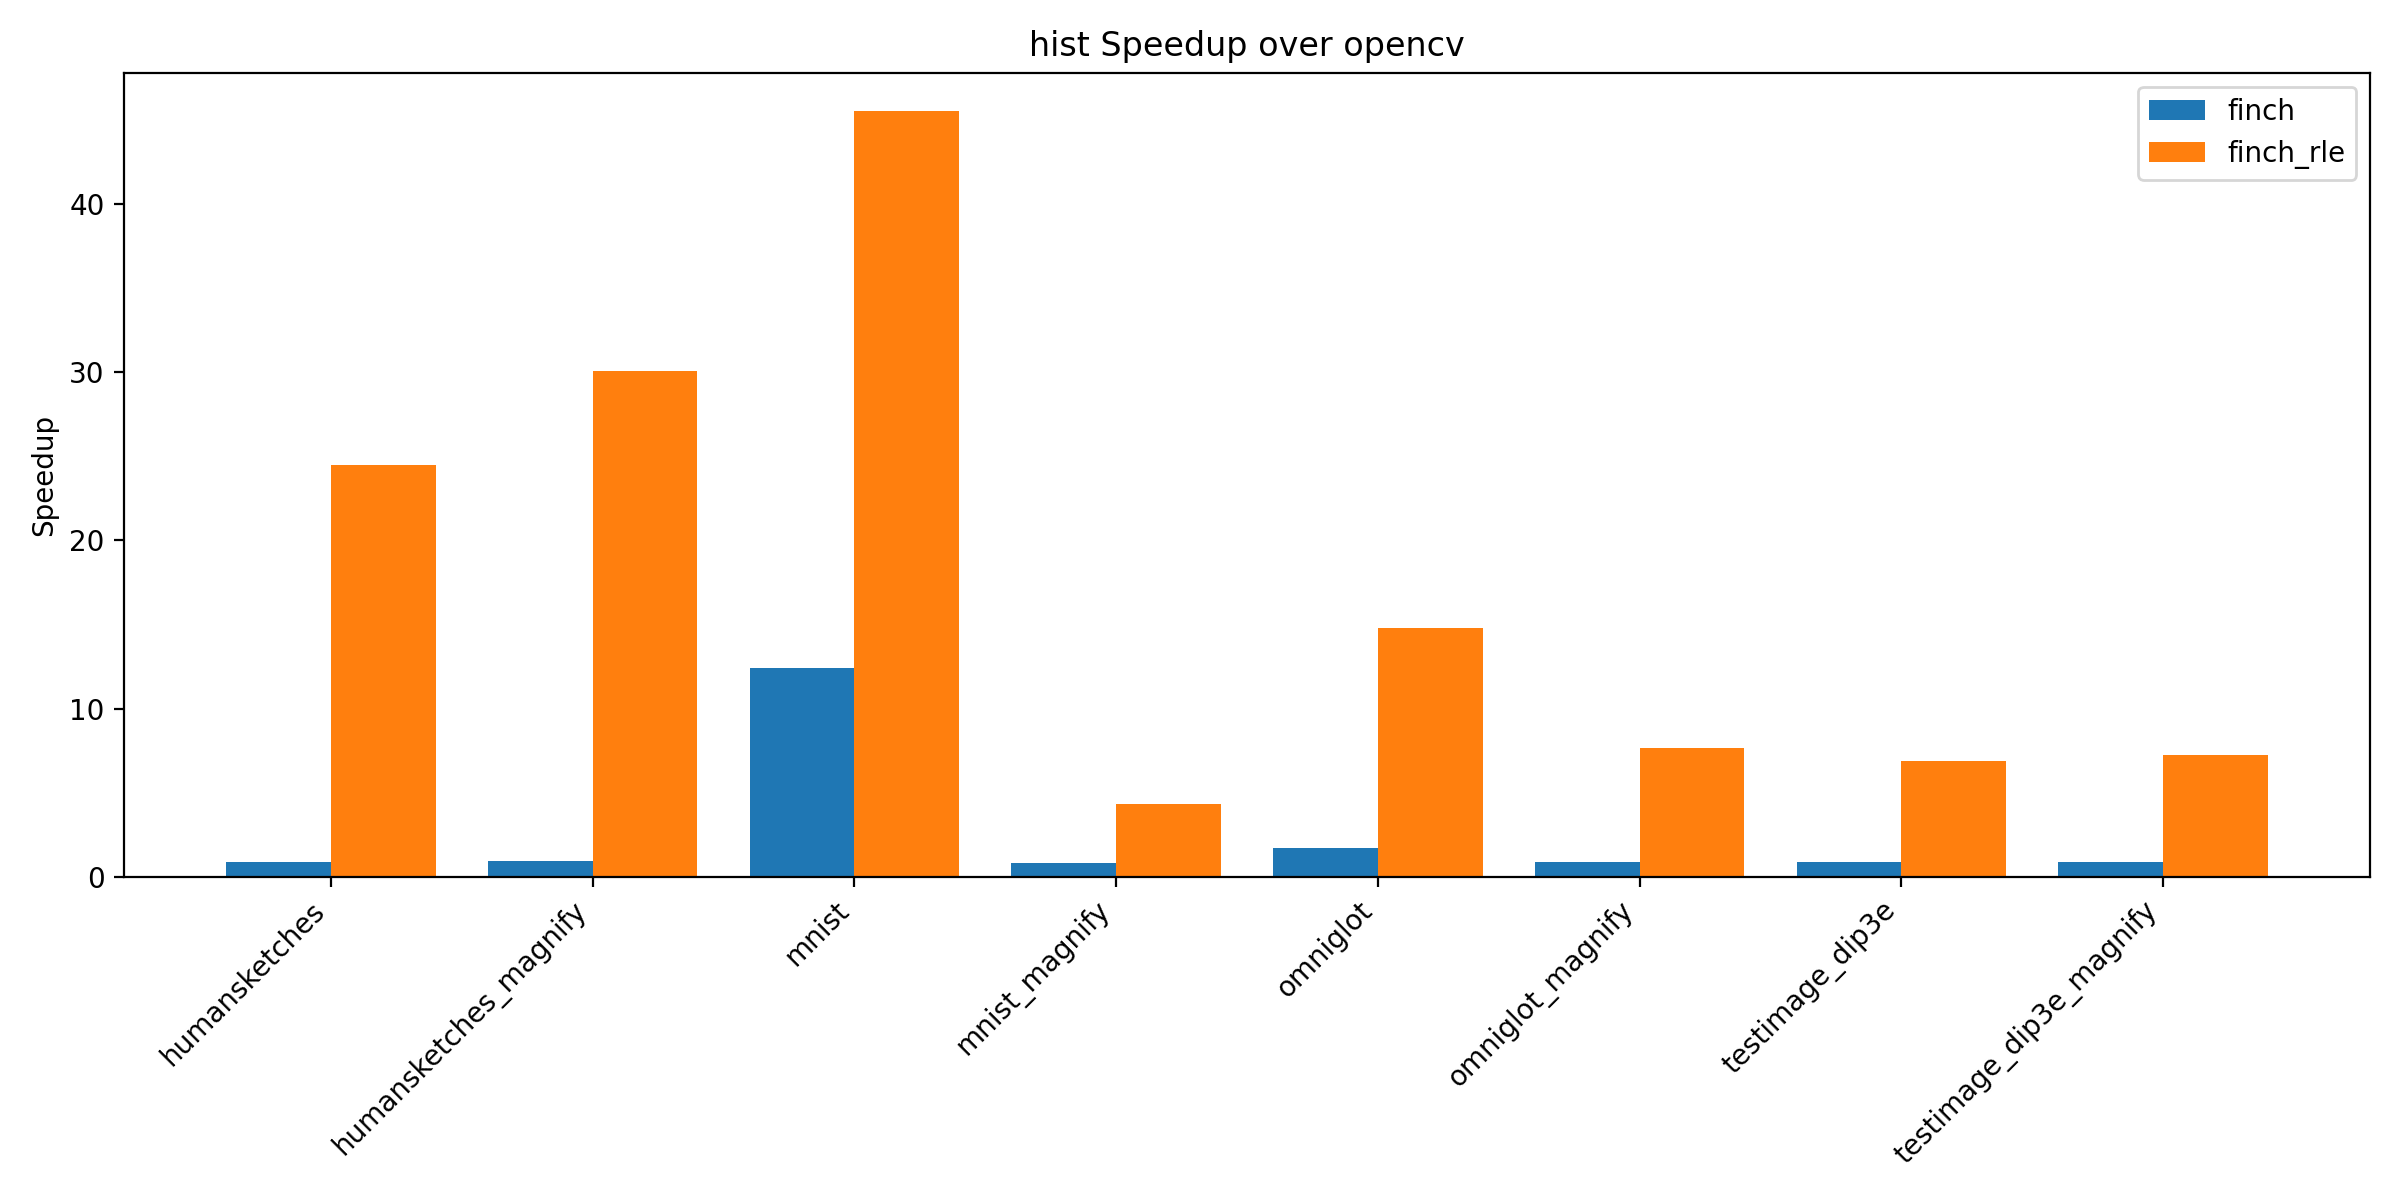
\includegraphics[width=\linewidth]{hist_speedup_over_opencv.png}
    \caption{Performance of Finch on masked histogram task.}
\end{figure}

\subsubsection{Graph Analytics}
\help{In this case, the two main highlights are that Finch can do arbitrary operators (i.e. choose), and that Finch can do early break, and also the different loop orders and multiple outputs. We may need to explain a little bit about what push pull is. For bellman, the main point is that we need multiple outputs, sparse inputs, masks, and sparse outputs with differing formats at differing points.}

\begin{figure}
	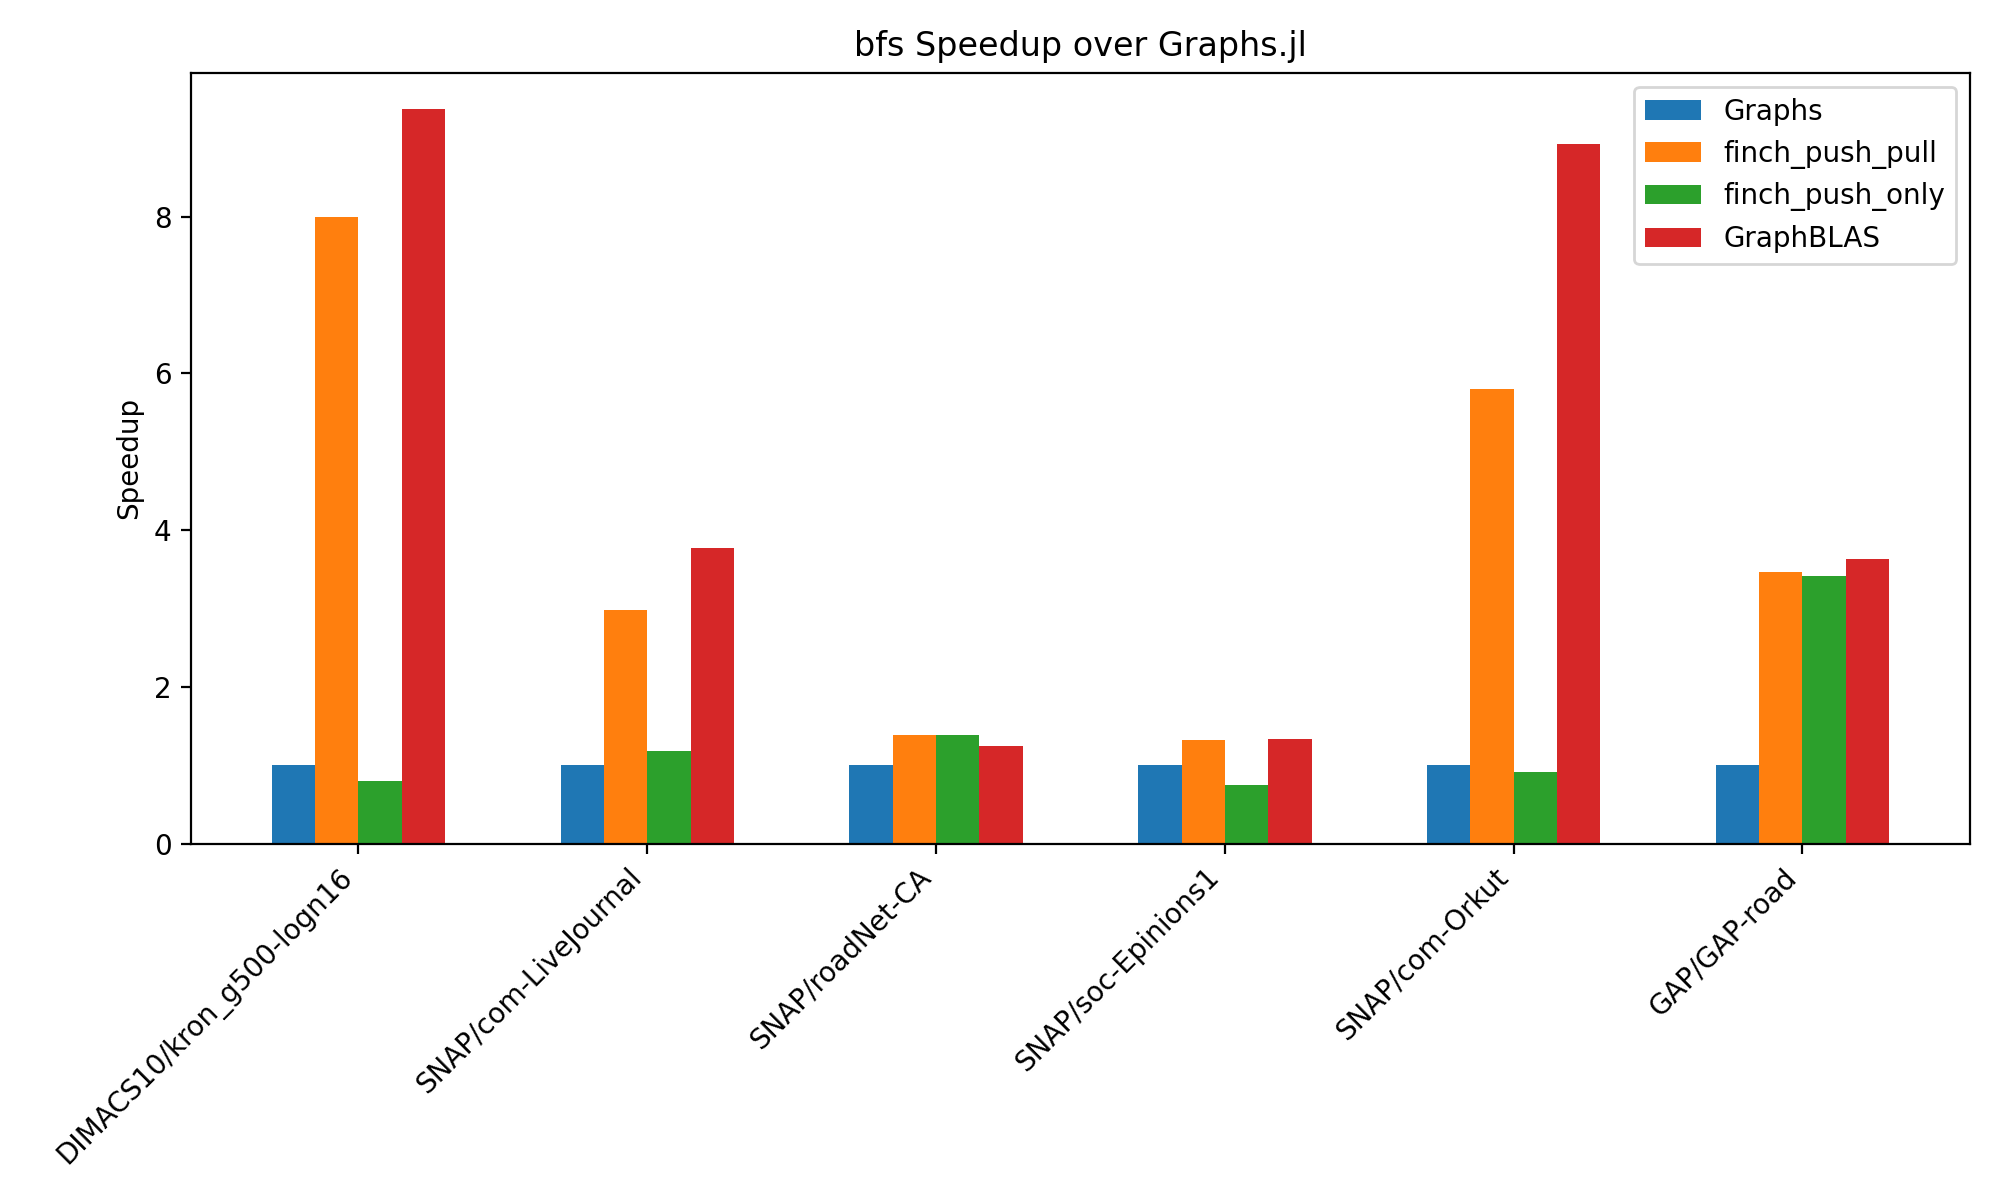
\includegraphics[width=\linewidth]{bfs_speedup_over_graphs.jl.png}
	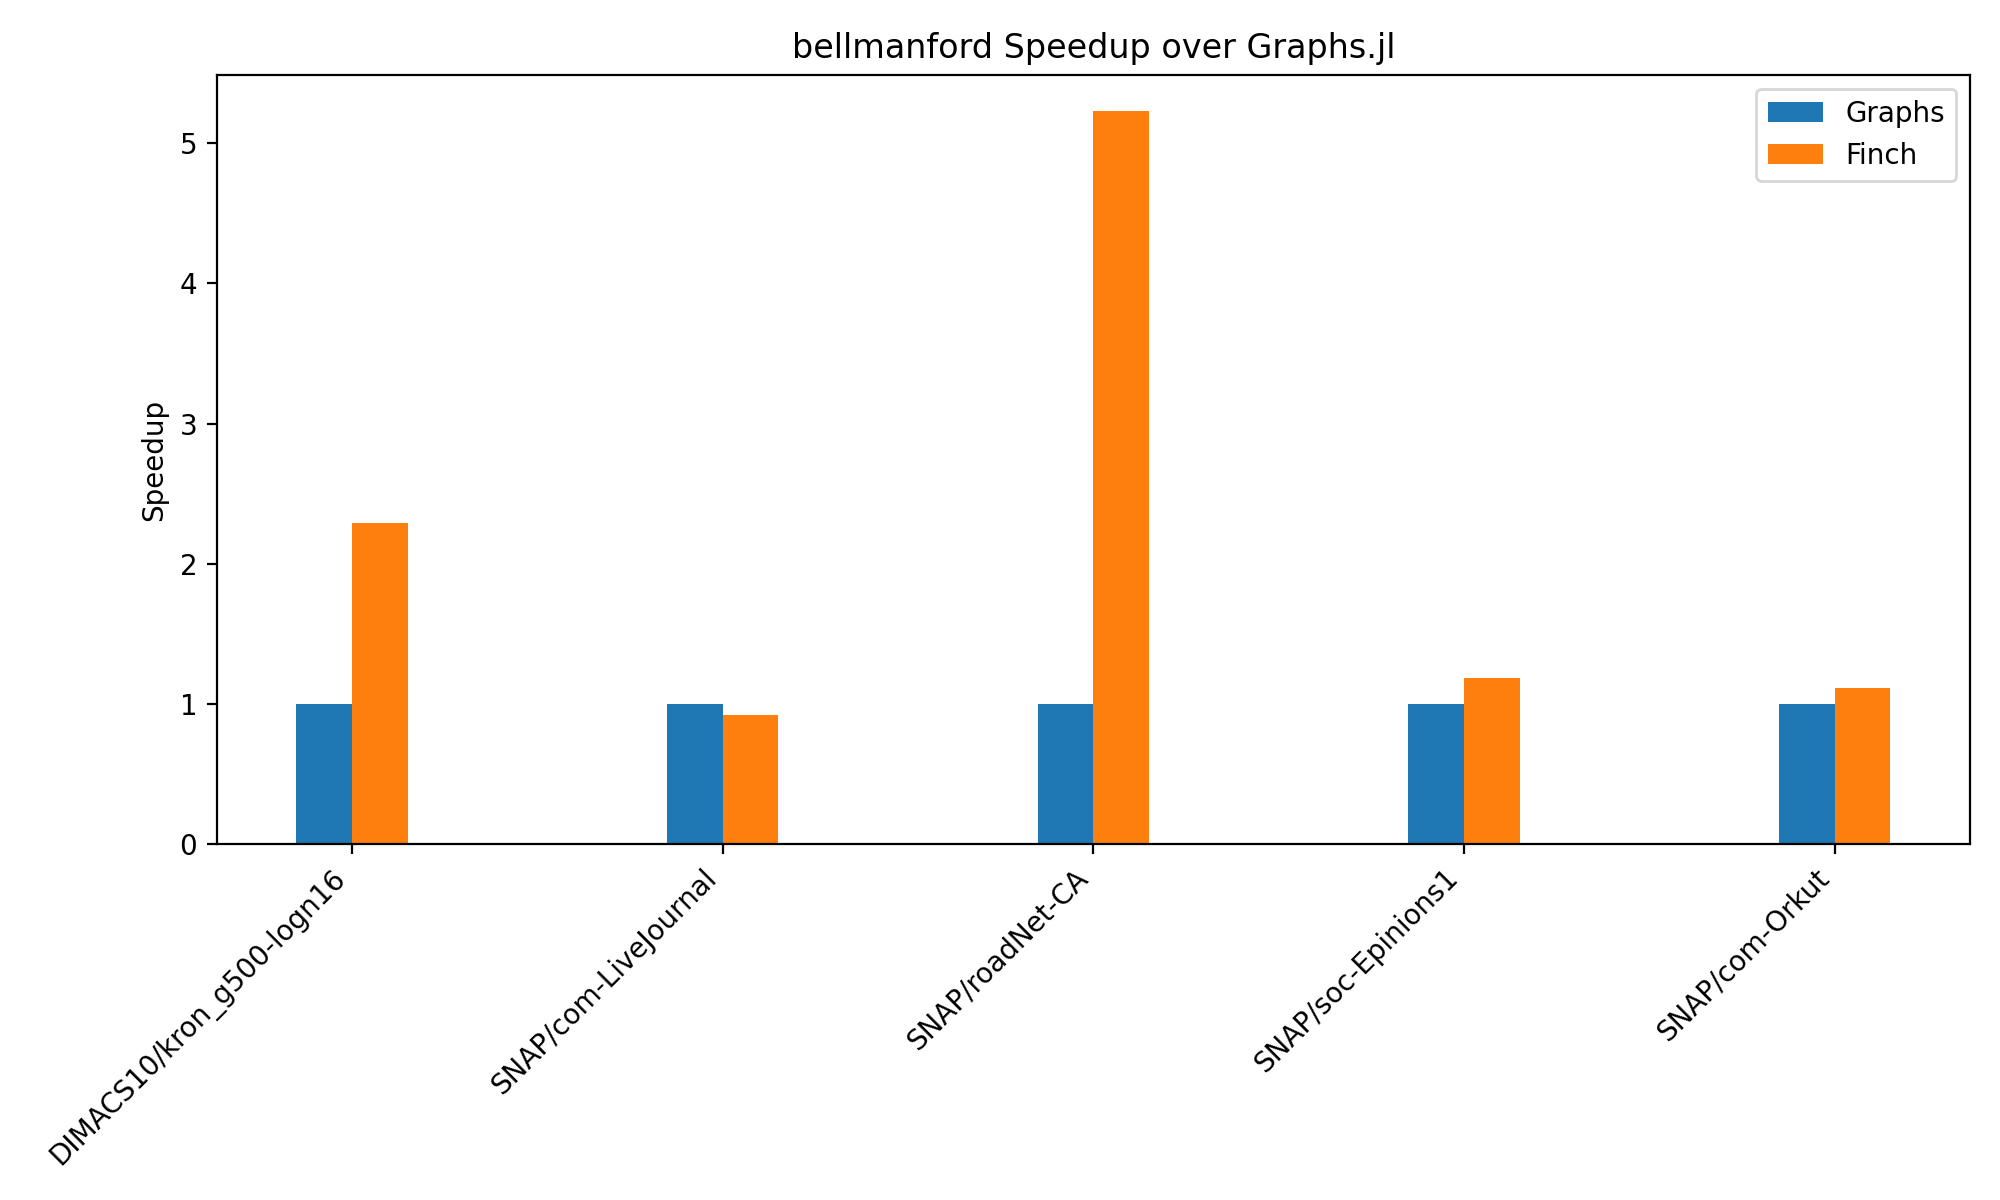
\includegraphics[width=\linewidth]{bellmanford_speedup_over_graphs.jl.png}
    \caption{Performance of graph apps across various tools.}
\end{figure}

Push-Pull BFS in Finch:
\begin{minted}{julia}
V = Tensor(Dense(Element(false)))
P = Tensor(Dense(Element(0)))
F = Tensor(SparseByteMap(Pattern()))
_F = Tensor(SparseByteMap(Pattern()))
A = Tensor(Dense(SparseList(Pattern())))
AT = Tensor(Dense(SparseList(Pattern())))

function finch_bfs_push_kernel(_F, F, A, V, P)
    @finch begin
        _F .= false
        for j=_, k=_
            if F[j] && A[k, j] && !(V[k])
                _F[k] |= true
                P[k] <<choose(0)>>= j #Only set the parent for this vertex
            end
        end
        return _F
    end
end


function finch_bfs_pull_kernel(_F, F, AT, V, P)
    p = ShortCircuitScalar{0}()
    @finch begin
        _F .= false
        for k=_
            if !V[k]
                p .= 0
                for j=_
                    if F[follow(j)] && AT[j, k]
                        p[] <<choose(0)>>= j #Only set the parent for this vertex
                    end
                end
                if p[] != 0
                    _F[k] |= true
                    P[k] = p[]
                end
            end
        end
        return _F
    end
end
\end{minted}

\subsection{Implementing Numpy Array API in Finch}


\subsubsection{The Finch High-Level API (Needs a Name)}

\subsubsection{Finch Logic}

\subsubsection{Finch Interpreter}

\subsubsection{Lowering}
\subsubsection{Heuristic Optimization}

Find an example where fusing the python interface gives a big speedup over non-fused kernels.

%matmul, mttkrp, repeated ttm, triangle counting, multiple pointwise,
%in-place.
%dot((v^t .* u), w)) vs. 
%(v^t .* dot(u, w))
